\documentclass[border=10pt]{standalone}
\usepackage{pgfplots}
\pgfplotsset{width=7cm,compat=1.8}
\usepackage{pgfplotstable}
\renewcommand*{\familydefault}{\sfdefault}
\usepackage{sfmath}

\begin{document}
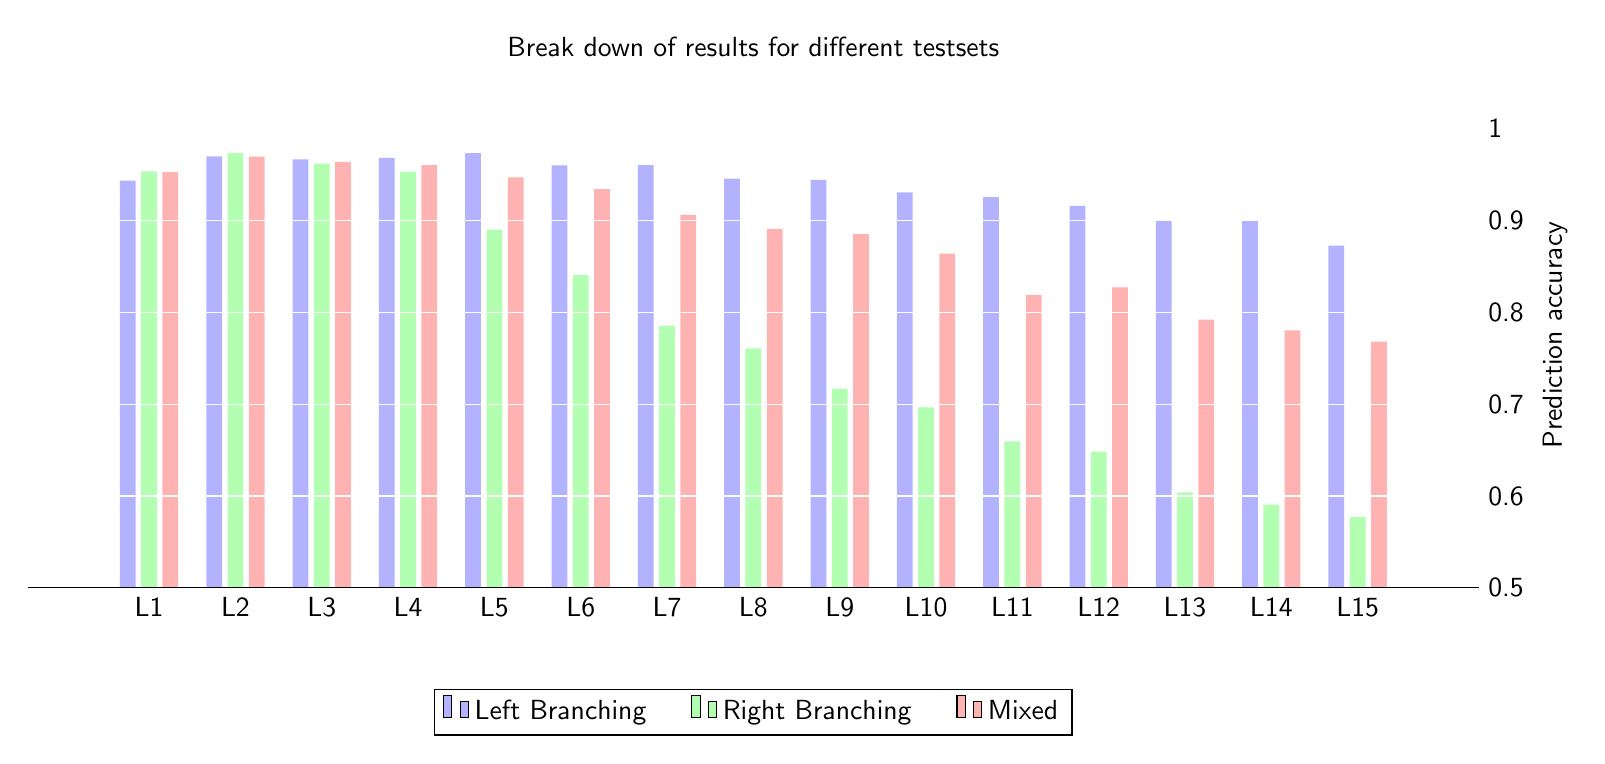
\begin{tikzpicture}
  \centering
  \begin{axis}[
        ybar, axis on top,
        title={Break down of results for different testsets},
        height=8cm, width=20cm,
        bar width=0.2cm,
        ymajorgrids, tick align=inside,
        major grid style={draw=white},
        enlarge y limits={value=.1,upper},
        ymin=0.5, ymax=1,
        axis x line*=bottom,
        axis y line*=right,
        y axis line style={opacity=0},
        tickwidth=0pt,
        enlarge x limits=true,
        legend style={
            at={(0.5,-0.2)},
            anchor=north,
            legend columns=-1,
            /tikz/every even column/.append style={column sep=0.5cm}
        },
        ylabel={Prediction accuracy},
        symbolic x coords={
            L1, L2, L3, L4, L5, L6, L7,
            L8, L9, L10, L11, L12, L13,
            L14, L15},
        xtick=data%,
       % nodes near coords={
        %\pgfmathprintnumber[precision=0]{\pgfplotspointmeta}
       %}
    ]
    \addplot [draw=none, fill=blue!30] coordinates {
        (L1, 0.94333333333333336)
        (L2, 0.96966666666666657)
        (L3, 0.96633333333333338)
        (L4, 0.96799999999999997)
        (L5, 0.97299999999999998)
        (L6, 0.95966666666666667)
        (L7, 0.95999999999999985)
        (L8, 0.94533333333333325)
        (L9, 0.94399999999999995)
        (L10, 0.93033333333333335)
        (L11, 0.92533333333333323)
        (L12, 0.91566666666666674)
        (L13, 0.89933333333333332)
        (L14, 0.89900000000000002)
        (L15, 0.87233333333333329)
    };

    \addplot [draw=none, fill=green!30] coordinates {
        (L1, 0.953333)
        (L2, 0.973000)
        (L3, 0.961667)
        (L4, 0.953000)
        (L5, 0.889667)
        (L6, 0.840333)
        (L7, 0.785000)
        (L8, 0.760667)
        (L9, 0.716667)
        (L10, 0.696333)
        (L11, 0.659333)
        (L12, 0.648333)
        (L13, 0.604000)
        (L14, 0.590667)
        (L15, 0.577333)
    };

    \addplot [draw=none, fill=red!30] coordinates {
        (L1, 0.95233333333333337)
        (L2, 0.96933333333333327)
        (L3, 0.96366666666666667)
        (L4, 0.95999999999999985)
        (L5, 0.94666666666666666)
        (L6, 0.93400000000000005)
        (L7, 0.90600000000000014)
        (L8, 0.89066666666666661)
        (L9, 0.8849999999999999)
        (L10, 0.86366666666666658)
        (L11, 0.81899999999999995)
        (L12, 0.82699999999999985)
        (L13, 0.79199999999999993)
        (L14, 0.78033333333333343)
        (L15, 0.76800000000000013) };

    \legend{Left Branching, Right Branching, Mixed}
  \end{axis}
  \end{tikzpicture}
\end{document}

